\documentclass{article}
\usepackage{blindtext}
\usepackage{listings}
\usepackage[english]{babel}
\usepackage{hyperref}
\usepackage{comment}
\usepackage[backend=biber, sorting=none]{biblatex}
\nocite{*}
\usepackage{xcolor}
\usepackage{subcaption}
\usepackage{graphicx}
\hypersetup{
    colorlinks,
    linkcolor={red!50!black},
    citecolor={blue!50!black},
    urlcolor={blue!80!black}
}
\addbibresource{sample.bib}

\usepackage{svg}
\usepackage{fancyhdr}
\usepackage{lipsum}

\pagestyle{fancy}
\headheight=14pt

\fancyhf{}
\font\myfont=cmr12 at 24pt
\lhead{\small{Faiella Ciro, Giannino Pio Roberto, Scovotto Luigi and Tortora Francesco}}
\rhead{\small{\thepage}}

\title{\textbf{\myfont Autonomous Vehicle Driving: Group 8}}
\author{\small{Faiella Ciro, Giannino Pio Roberto, Scovotto Luigi and Tortora Francesco}}
\date{\small{\{\href{mailto:c.faiella8@studenti.unisa.it}{c.faiella8}, \href{mailto:p.giannino@studenti.unisa.it}{p.giannino}, \href{mailto:l.scovotto1@studenti.unisa.it}{l.scovotto1}, \href{mailto:f.tortora21@studenti.unisa.it}{f.tortora21}\}@studenti.unisa.it}}

\makeindex

\begin{document}
\maketitle
\centerline{\small{Jun, 2023}}
\centerline{Department of Computer Engineering, Electrical Engineering and Applied}
\centerline{Mathematics (DIEM), University of Salerno, Fisciano, Italy}
\newpage
\tableofcontents
\newpage
\section{Introduction}
The project focuses on the creation of an autonomous driving system to be included in the CARLA simulator 
environment. Unlike the task performed in the real world, in this case there is full knowledge of the world 
in which the vehicle is located, nevertheless the system has to face several challenges in order to avoid 
errors. 

\subsection{Development environment}
\subsubsection{Hardware}
We conducted the software testing on a Dell machine equipped with an NVIDIA Quadro P2000 graphics card, boasting 4GB of dedicated memory. 
The system was powered by an Intel 8th generation i9 processor, delivering exceptional processing power. Furthermore, it was equipped with a 
substantial 16GB of RAM, ensuring smooth and efficient operation throughout the testing phase.

\subsubsection{How we optimised the performance?}
In order to optimize performance and enhance the execution speed, we opted to remove all unnecessary sensors from the machine, 
as they were not utilized during the testing process. Leveraging our comprehensive global knowledge of the surrounding environment, 
we were able to confidently eliminate these redundant components. 
As a result, the execution speed experienced a notable improvement, exhibiting an impressive 30\% increase compared to the performance of
the machine with all the sensors on.

\subsubsection{CARLA Simulator}
The version of Carla used for this project is 0.9.13, which is launched via the carla simulator leaderboard 2.0.
The simulator is launched with the following command: 
\begin{lstlisting}[language=Bash]
    ./CarlaUE4.sh -quality-level=Low -prefernvidia
\end{lstlisting}
The parameter \textit{-quality-level=Low} is used to reduce the quality of the graphics, in order to increase the 
performance of the simulator. \textit{-prefernvidia} is used to force the use of the NVIDIA graphics card, if present, so we ensure the usage of our NVIDIA Quadro P2000.


\subsection{Task}
The CARLA AD Leaderboard challenges AD agents to drive through a series of predefined routes. For each route, 
agents are initialized at a starting point and directed to a destination point with a route description. 
Routes are defined in a variety of situations, including urban areas, residential neighborhoods and rural environments. 
The classification evaluates AD agents in different weather conditions, including daytime scenes, sunset, rain, fog and night.

\subsection{Baseline provided}
The baseline provided by the CARLA team is a simple agent that drives at a constant speed, follows the lane and stops at the traffic lights.
The agent is not able to handle the following situations:
\begin{itemize}
    \item overtakes of other vehicles;
    \item overtakes of obstacles;
    \item stops at stop signs;
    \item manage intersections;
    \item manage lane invasion;
    \item stop when a vehicle is parked or slow moving in roadside;
\end{itemize}

You can see a video of the baseline agent at the following link: \url{https://youtu.be/BLABLABLA}.

FARE VIDEO
\section{Operational Design Domain}
First of all, considering the fact that the data used by the ego-vehicle are directly provided by CARLA simulator and they are not took by any kind of sensor, we have 
that the our ODD has reached the following operational domains:
\begin{itemize}
    \item the vehicle is able to maintain the selected speed, thanks the longitudinal control;
    \item the vehicle is able to maintain the correct position between the lanes of a road thanks to the lateral control;
    \item the vehicle is able to manage its speed in according to the variable traffic conditions;
    \item the vehicle is able to avoid collisions with the car ahead if asphalt conditions are optimal and adapts its speed in order to follow that one;
    \item the vehicle is capable of overtaking when possible and when necessary;
    \item the vehicle is capable to makes an emergency stop when a pedestrian or a cyclist is detected in front of it in time;
    \item the vehicle is able to operate in sunny, foggy and poor lighting environments, but in presence of rain it is not always able to operate correctly;
    \item the vehicle can operate in urban and non-urban contexts;
    \item the vehicle is capable of handling junctions;
    \item the vehicle is able to avoid collisions with obstacles that can be find through the path (e.g. road cones, traffic sign, construction obstacle, etc.);
    \item the vehicle is able to correctly pass the traffic light;
    \item the vehicle is able to elude vehicles that invade its lane;
\end{itemize}

\subsection{Traffic Scenario}
Agents will experience multiple instances of traffic scenarios selected from the NHTSA pre-crash typology \cite{NHTSA}. 
\newpage
\subsubsection{Control loss}
The ego-vehicle loses control due to bad conditions on the road and it must recover, coming back to its original lane.
\begin{figure}[h]
    \centering
    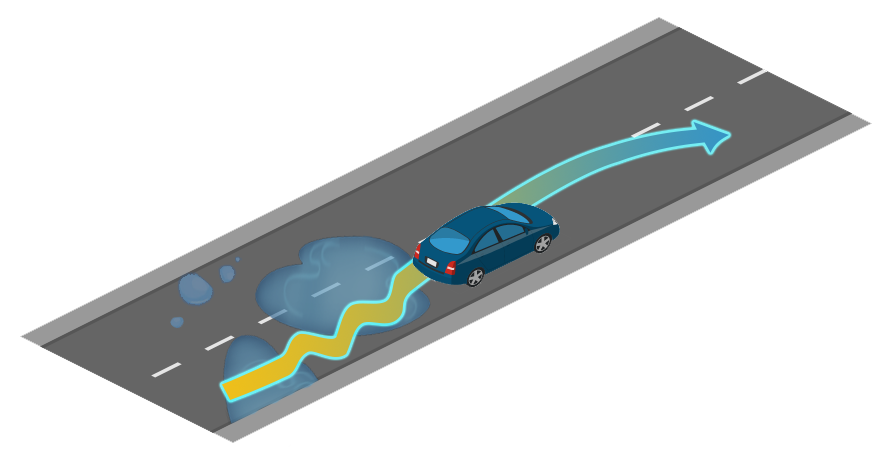
\includegraphics[width=0.5\textwidth]{img/TR01.png}
    \caption{Control loss without previous action} \label{Scenario_controlLoss}
\end{figure}

\subsubsection{Traffic negotiation}
\textbf{Unprotected left turn at intersection with oncoming traffic}
The ego-vehicle is performing an unprotected left turn at an intersection, yielding to oncoming traffic. This scenario occurs at both signalized and non-signalized junctions.
\begin{figure}[h]
    \centering
    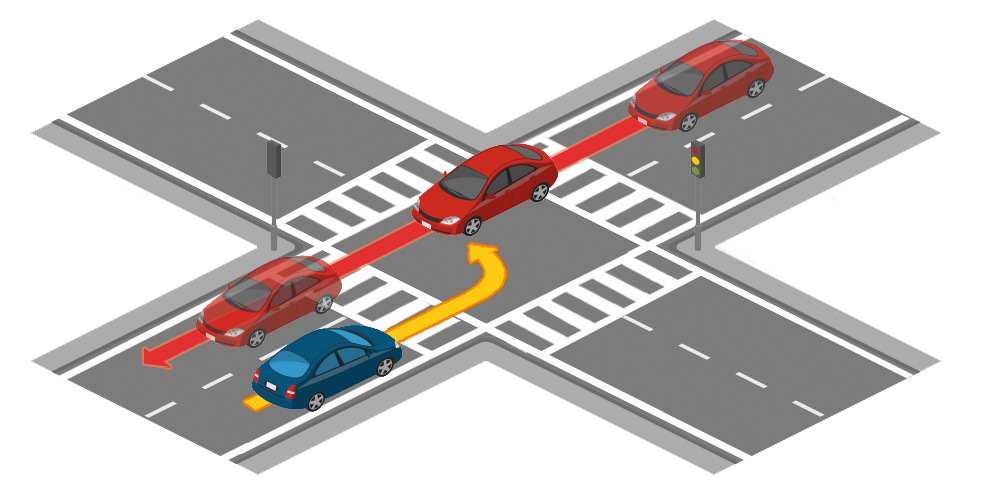
\includegraphics[width=0.5\textwidth]{img/TR08.png}
    \caption{Unprotected left turn at intersection with oncoming traffic} \label{leftTurn}
\end{figure}

\textbf{Right turn at an intersection with crossing traffic} 
The ego-vehicle is performing a right or left turn at an intersection, yielding to crossing traffic. This scenario occurs at both signalized and non-signalized junctions.
\begin{figure}[h]
    \centering
    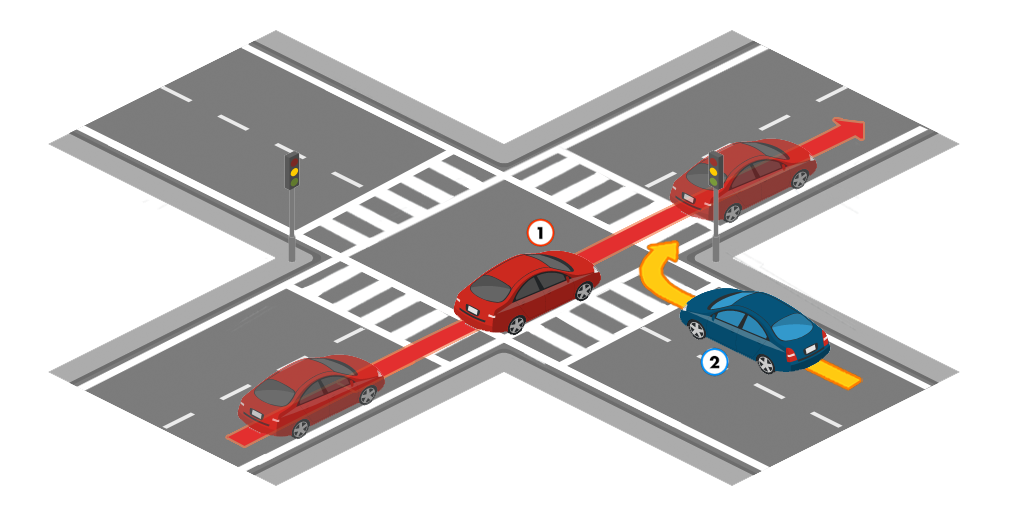
\includegraphics[width=0.5\textwidth]{img/TR09.png}
    \caption{Right turn at an intersection with crossing traffic} \label{rightTurn}
\end{figure}

\subsubsection{Obstacle avoidance}
\textbf{Obstacle in lane} 
The ego-vehicle encounters an obstacle blocking the lane and must perform a lane change into traffic moving in the opposite direction to avoid it. 
The obstacle may be a construction site, an accident or a parked vehicle.
\begin{figure}[h]
    \centering
    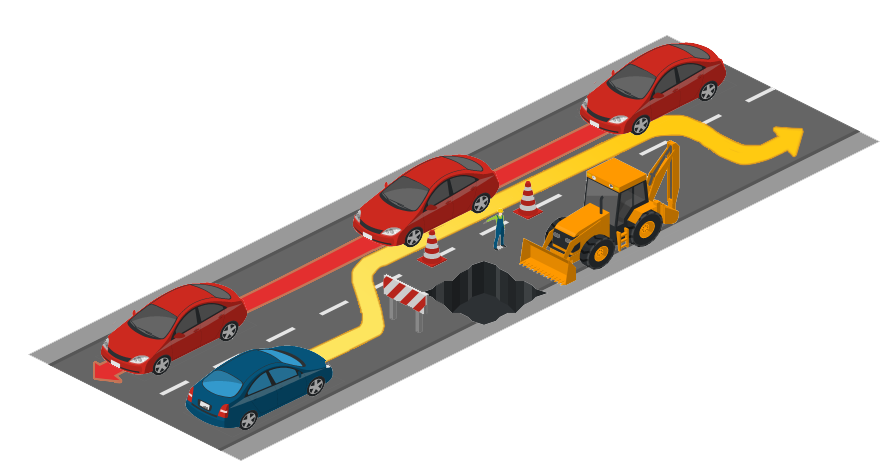
\includegraphics[width=0.5\textwidth]{img/TR14a.png}
    \caption{Obstacle in lane} \label{Scenario_obstacle}
\end{figure}

\textbf{Slow moving hazard at lane edge} 
The ego-vehicle encounters a slow moving hazard blocking part of the lane. The ego-vehicle must brake or maneuver to avoid it next to a lane of traffic 
moving in the opposite direction.
\begin{figure}[h]
    \centering
    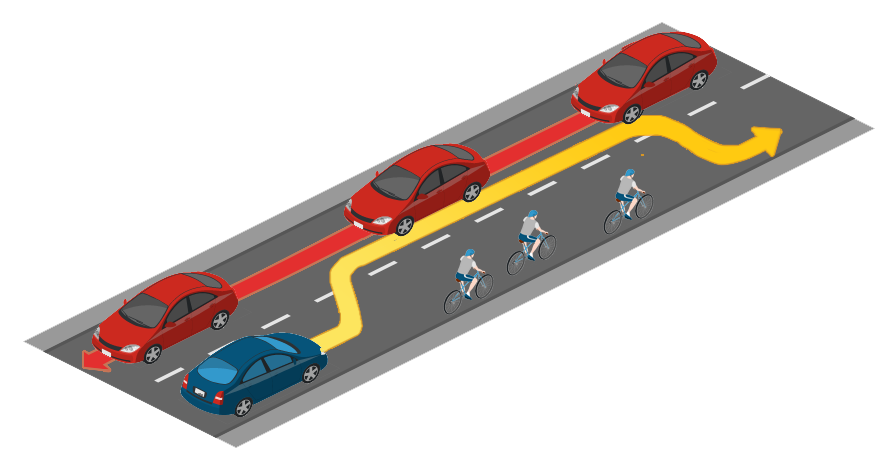
\includegraphics[width=0.5\textwidth]{img/TR16a.png}
    \caption{Slow moving hazard at lane edge} \label{Scenario_slowMove}
\end{figure}

\textbf{Vehicle invading lane on bend} 
The ego-vehicle encounters an oncoming vehicles invading its lane on a bend due to an obstacle. It must brake or maneuver to the side of the road 
to navigate past the oncoming traffic.
\begin{figure}[h]
    \centering
    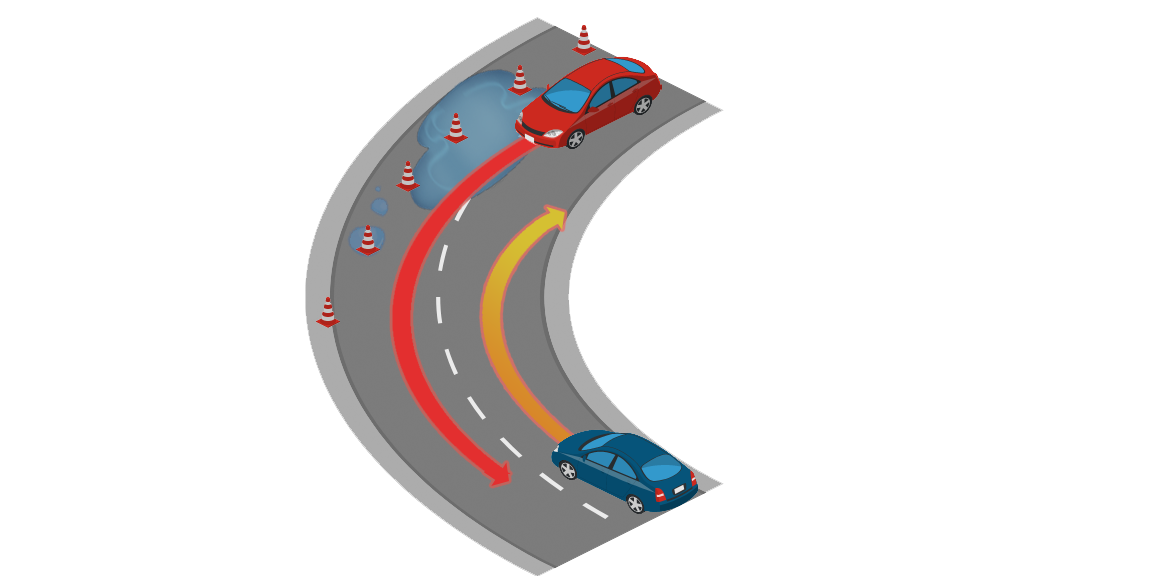
\includegraphics[width=0.5\textwidth]{img/TR22.png}
    \caption{Vehicle invading lane on bend} \label{Scenario_vehicleInvading}
\end{figure}

\subsubsection{Braking and lane changing}
\textbf{Longitudinal control after leading vehicle’s brake} 
The leading vehicle decelerates suddenly due to an obstacle and the ego-vehicle must perform an emergency brake or an avoidance maneuver.
\begin{figure}[h]
    \centering
    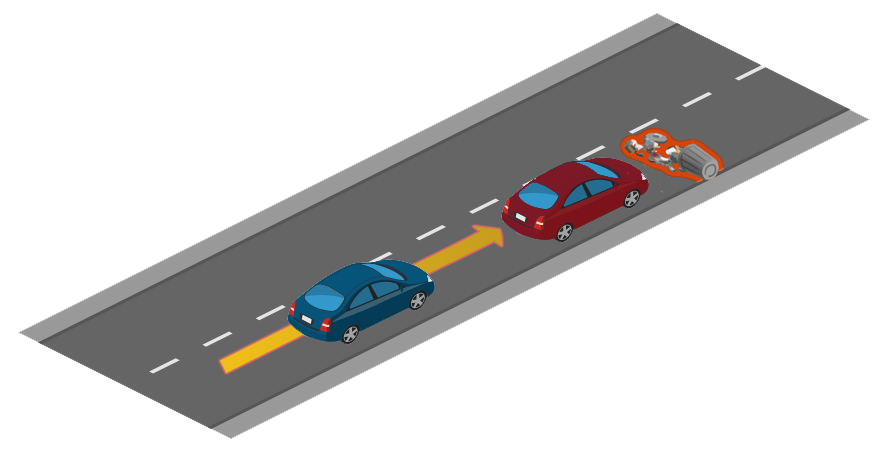
\includegraphics[width=0.5\textwidth]{img/TR02.png}
    \caption{Longitudinal control after leading vehicle’s brake} \label{Scenario_longgitudinalControl}
\end{figure}

\textbf{Obstacle avoidance without prior action} 
The ego-vehicle encounters an obstacle / unexpected entity on the road and must perform an emergency brake or an avoidance maneuver.
\begin{figure}[h]
    \centering
    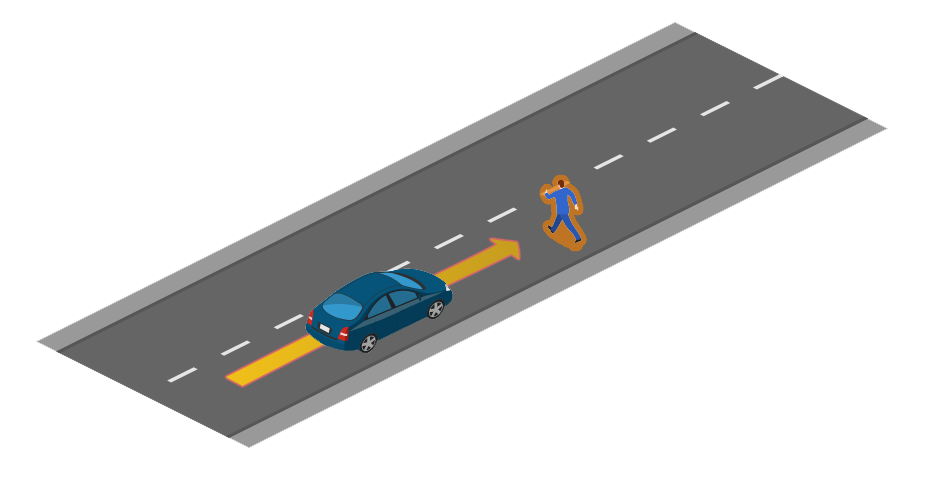
\includegraphics[width=0.5\textwidth]{img/TR03.png}
    \caption{Obstacle avoidance without prior action} \label{Scenario_obsAvoidanceWithout}
\end{figure}

\textbf{Pedestrian emerging from behind parked vehicle} 
The ego-vehicle encounters an pedestrian emerging from behind a parked vehicle and advancing into the lane. The ego-vehicle must brake or maneuver to avoid it.
\begin{figure}[h]
    \centering
    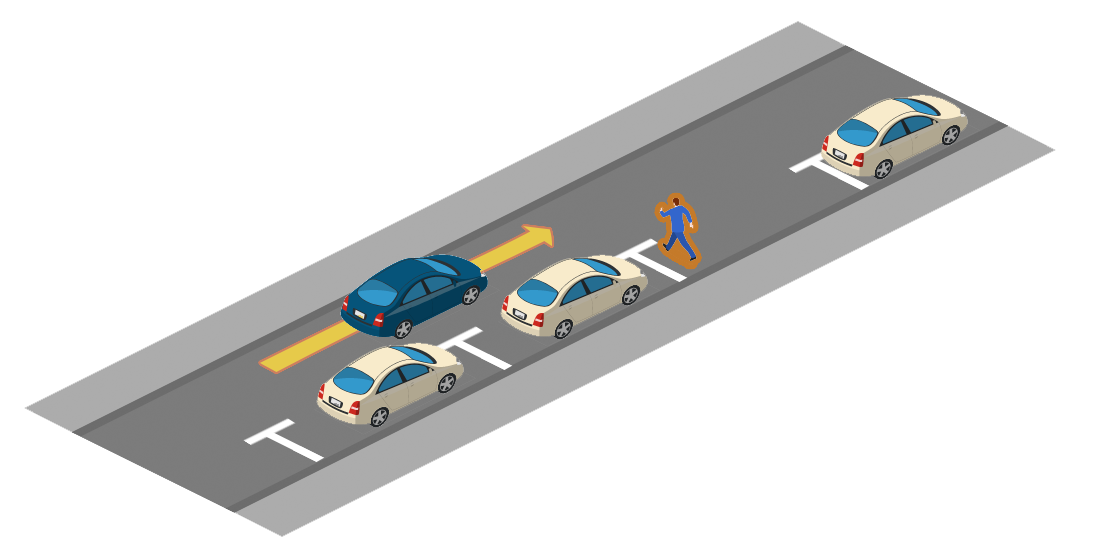
\includegraphics[width=0.5\textwidth]{img/TR17.png}
    \caption{Pedestrian emerging from behind parked vehicle} \label{Scenario_pedestrianEmerging}
\end{figure}

\textbf{Obstacle avoidance with prior action - pedestrian or bicycle} 
While performing a maneuver, the ego-vehicle encounters an obstacle in the road, either a pedestrian or a bicycle, and must perform an emergency brake 
or an avoidance maneuver.
\begin{figure}[h]
    \centering
    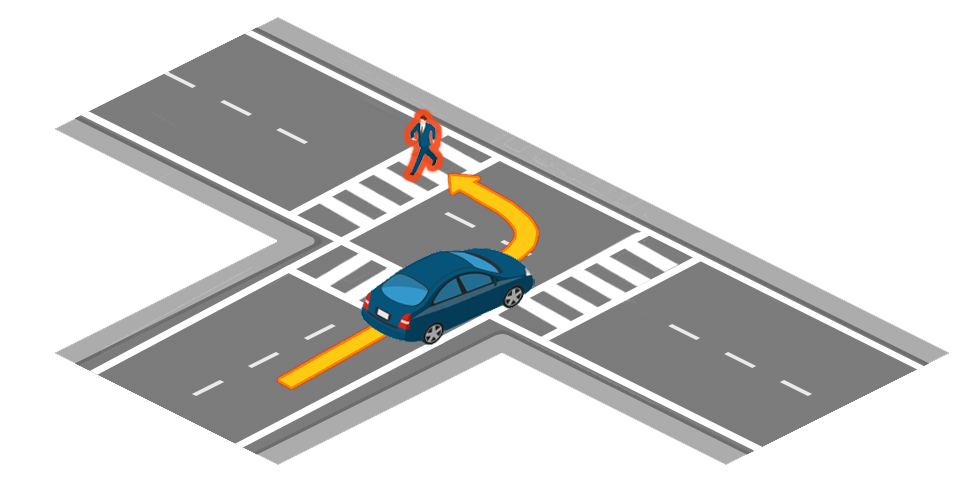
\includegraphics[width=0.5\textwidth]{img/TR04.png}
    \caption{Obstacle avoidance with prior action - pedestrian or bicycle} \label{Scenario_obsAvoidanceWithPedBic}
\end{figure}

\textbf{Obstacle avoidance with prior action - vehicle} 
While performing a maneuver, the ego-vehicle encounters a stopped vehicle in the road and must perform an emergency brake or an avoidance maneuver.
\begin{figure}[h]
    \centering
    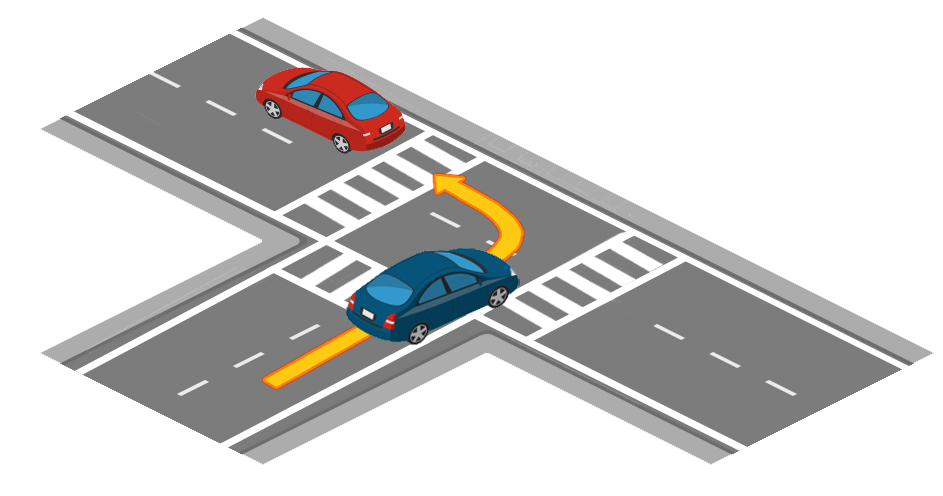
\includegraphics[width=0.5\textwidth]{img/TR19a.png}
    \caption{Obstacle avoidance with prior action - vehicle} \label{Scenario_obsAvoidanceWithoutVehicle}
\end{figure}

\section{Vehicle configuration}
The vehicle used for the project is the default vehicle provided by CARLA. 
This vehicle has automatic transmission and is not provided of sensors because we have not used them as we have full knowledge of the environment.
\section{Evaluation and metrics}
The driving proficiency of an agent can be characterized by multiple metrics. For the assigned leaderboard, we have a number of metrics that help 
to understand different aspects of driving. Although all routes have the same type of metrics, the respective values are calculated separately. 
The specific metrics are as follows:
\begin{itemize}
  \item \textbf{Driving score}: main metric of the leaderboard, serving as the product between the route completion and the infractions penalty, $R_i * P_i$.
  Here \textit{Ri} is the percentage of completion of the \textit{i-th} route, and \textit{Pi}, 
  the infraction penalty of the \textit{i-th} route;
  \item \textbf{Route completion}: percentage of the route completed by the agent;
  \item \textbf{Infraction penalty}: productory of the infractions committed,

  
  $\prod_{j}^{ped., ..., stop} (a_{\small{i}}^{\small{j}})^{\small{\#infractions}_j}$. — 
  The leaderboard tracks several types of infractions and this metric aggregates all of these infractions triggered by an agent as a geometric series. Agents start with an ideal 1.0 
  base score, which is reduced each type an infraction is committed.
\end{itemize}
When all routes have been completed, a global metric for each of the previous three types is also generated, being the arithmetic mean of all the individual routes combined. 
The global driving score is the main metric on which you will be classified with respect to other participants.

\subsection{Infractions and shutdown events}
The CARLA leaderboard offers individual metrics for a series of infractions. Each of these has a penalty coefficient that will be applied everytime it happens. 
The infractions are the following:
\begin{itemize}
    \item \textbf{Collisions with pedestrians} - $a_{\small{i}}^{\small{ped.}} = 0.60$
    \item \textbf{Collisions with vehicles} - $a_{\small{i}}^{\small{veh.}} = 0.50$
    \item \textbf{Collisions with static elements} - $a_{\small{i}}^{\small{statEl.}} = 0.65$
    \item \textbf{Running a red light } - $a_{\small{i}}^{\small{light.}} = 0.70$
    \item \textbf{Stop sign} - $a_{\small{i}}^{\small{stop.}} = 0.80$
    \item \textbf{Scenario timeout} - $a_{\small{i}}^{\small{time.}} = 0.70$. Some scenarios feature behaviors that can block the ego-vehicle indefinitely. 
            These scenarios will have a timeout of 4 minutes after which the ego-vehicle will be released to continue the route. However, a penalty is applied when 
            the time limit is breached.
    \item \textbf{Failure to maintain minimum speed} - $a_{\small{i}}^{\small{speed.}} = 0.70$. The agent is expected to maintain a minimum speed in keeping with nearby traffic.
            The agent’s speed will be compared with the speed of nearby vehicles. Failure to maintain a suitable speed will result in a penalty.
    \item \textbf{Failure to yield to emergency vehicle} - $a_{\small{i}}^{\small{yield.}} = 0.70$. The agent should yield to emergency vehicles coming from behind. Failure to allow the emergency vehicle to pass will incur a penalty.
    \item \textbf{Off-road driving} - If an agent drives off-road, that percentage of the route will not be considered towards the computation of the route completion score.
\end{itemize}

Additionally, some events will interrupt the simulation, preventing the agent to continue. In these cases, the route which is being simulated will be shut down, and the 
leaderboard will move onto the next one, triggering it normally.
\begin{itemize}
    \item \textbf{Route deviation} — If an agent deviates more than 30 meters from the assigned route.
    \item \textbf{Agent blocked} — If an agent doesn’t take any actions for 180 simulation seconds.
    \item \textbf{Simulation timeout} — If no client-server communication can be established in 60 seconds.
    \item \textbf{Route timeout} — If the simulation of a route takes too long to finish.
\end{itemize}

\section{Project development and phases }
In this section we will explain how we handled certain situations that occurred in the routes, 
in order to show the level of attention achieved by our system.

The main problems were determined in order to define the problem domain. 
From there, we moved on to the development of solutions, first developing the problems that first appeared on the routes.
\subsection{Controllers}
One of the first tasks was the configuration of the controller, in order to determine a driving behavior that 
would seem as natural as possible. 
\subsubsection{PID Controller}
The PID controller was configured on the basis of several initial attempts. They led to the following values:
$$"longitudinal\_control\_dict" : {"K_P": 0.888 , "K_I": 0.0768, "K_D": 0.05, "dt": 0.05}$$

\subsubsection{Stanley Controller}
The same approach, but different methodology, was used for the Stanley controller configuration:
$$"lateral\_control\_dict" : {"K_V": 4, "K_S": 1, "dt": 0.05}$$

\subsection{Obstacle avoidance and overtake}
The development of the overtaking manoeuver was one of the most challenging tasks due to its importance 
within such a system; its difficulty was such that it required constant development of this feature during 
the course of the entire project. The solution found is optimal, with no errors in the management of the 
various events.

\subsubsection*{Previous checks}\label{checkover}
We do different checks for the overtake of a vehicle and an obstacle.

If we have to overtake a vehicle, we check whether it is possible to overtake it in the following way:
\begin{itemize}
    \item check if the lane is broken or solid-broken;
    \item check if we are not already overtaking;
    \item check if we are near the following vehicle;
    \item check if the direction is "LANEFOLLOW";
    \item check if the vehicle in front of us is slow;
    \item check if in the other lane there is a vehicle;
    \item check if we are in proximity of a junction.
\end{itemize}

If we have to overtake an obstacle, we check whether it is possible to overtake it in the following way:
\begin{itemize}
    \item check if our speed is near to zero;
    \item check if the lane is broken or solid-broken;
    \item check if in the other lane there is a vehicle;
\end{itemize}

\subsubsection*{Calculate the total distance of the overtake}
We developed a function that calculates the total distance of the overtake.
It consists in counting the number of vehicles in front which have as their distance from each other max 15 meters. 
So we know the total distance of the overtake, the number of vehicles in front of, the distance between each vehicle.
This method is really important for the previous checks and for the lane change.

\subsubsection*{Lane change}
In order to create a path that allow the ego-vehicle to change lane, here's the logic we used:
we generates a path to perform a lane change in a controlled manner. It uses the given parameters to 
calculate the distance to the same lane, to the target lane and to the lane change. It then creates 
the path that crosses these distances, taking into account the required directions and checking the 
availability of lanes. 

Finally, it returns the complete route. In the event of errors or inability to 
perform the lane change, we returns an empty route. In short, this function facilitates safe and 
controlled lane changes.

\subsubsection*{A clarification} We save the path before overtaking and, once we have finished, we take the saved path, 
delete the points that are not needed (so the points preceding the return of the overtaking) and use it
to follow the initial path.

\subsubsection*{Overtaking manoeuver}
The logic of the overtake is the following:
first, if the agent is terminating an overtaking manoeuver, actions are performed to complete the overtaking and 
re-enter the original lane. If the agent is in the process of overtaking, actions are performed to continue 
overtaking and to check the possibility of re-entering the original lane. In both cases, the target speed 
is set and the local planner is executed to obtain driving control.

\subsection{Stop sign and Traffic negotiation}
Another phase concerned the management of stops; after trying countless solutions, we arrived at a solution that 
uses the static \textit{*stop*}. What we do, is to take all the stops in the scenario and evaluate whether they 
affect the ego-vehicle. 
Management begins by taking all stop signals and putting them into a listings, then the system follows these steps:
\begin{enumerate}
    \item for each stop sign, evaluate the distance between the stop sign and the ego-vehicle and discarding all distant stops;
    \item sort the remaining stops by the minimum distance and not consider those we have already passed;
    \item check all vehicles coming from the right and left.
\end{enumerate}
Now we have all the information that we needed, so the ego-vehicle follows this behavior:
\begin{itemize}
    \item if there is no vehicle in the left and right lane, the stop sign is not affecting the vehicle;
    \item if there is a vehicle in the left lane, check if it is still affecting the vehicle;
    \item if there is a vehicle in the right lane, check if it is still affecting the vehicle;
    \item otherwise, the ego-vehicle can go.
\end{itemize}

\subsection{Other vehicles invading the ego lane}
There was also a phase where we handled lane invasion, since there are lane restrictions within the routes. 
The solution to this problem is the following:
\begin{enumerate}
    \item Check if an invasion is detected and calculate the distance between the center of the vehicle that invaded our lane and his waypoint;
    \item The vehicle performs a deceleration and moves sideways, moving at the distance calculated before, to avoid the invasion; 
    \item The target speed is reduced to ensure safe driving during this manoeuver;
    \item Once the expansion disappears, the vehicle returns to its normal driving position by restoring the lateral offset and resuming the target speed. 
\end{enumerate}
These measures allow the vehicle to react appropriately and safely to lane-change situations.

\subsection{Pedestrian avoidance behaviors}
The management of vehicle behavior in the presence of pedestrians was partly carried out, 
although there was not enough time for full development of the solution. 
We check if a pedestrian is on our lane and, if so, appropriate actions are taken to avoid a collision. 
The distance between the vehicle and the pedestrian is calculated taking into account the size of the 
respective bounding boxes.  
\begin{itemize}
    \item If the distance is less than the vehicle's braking distance, an emergency brake is executed to avoid an imminent collision;
    \item If the distance is less than 15 metres, an emergency brake is also executed. 
\end{itemize}
These measures allow the vehicle to react quickly and effectively to the presence of pedestrians on the road, 
ensuring safety for both vehicle driver and pedestrians.

\section{Qualitative analysis of results}
\subsection{Video}
We did six video:
\begin{itemize}
    \item \textbf{Baseline agent}: In this video we show the behavior of the baseline agent in all the routes. \url{https://youtu.be/BLABLABLA}
    \item \textbf{Full video}: In this one we show the behavior of our agent in all the routes. \url{https://youtu.be/RBGWd_so80U}
    \item \textbf{Overtakes}: In this video we show all the overtakes. \url{https://youtu.be/vDg-9poUQ9k}
    \item \textbf{Vehicle invading lane on bend}: In this video we show all the lane invasions. \url{https://youtu.be/KME91FAB5ko}
    \item \textbf{Traffic negotiation}: In this video we show all the traffic negotiation. \url{https://youtu.be/d2ESc0bXmmg}
    \item \textbf{Simulator errors} In this video we show all the errors caused by the simulator. \url{https://youtu.be/0O9b3UihDAw}
\end{itemize}
scrivere dove siamo arrivati mostrando i video (minuti) e fare il confronto tra prima e dopo l'ottimizzazione
\subsection{Control loss}
Since neither the traction control system nor ABS has been implemented, impacts may occur due to wet or dirty road conditions, 
resulting in loss of vehicle control. Nevertheless, if the braking distance exceeds a certain threshold, impacts will not occur as 
indicated in the minute 10:35 of the \href{https://youtu.be/RBGWd_so80U?t=635}{main video}. Due to the lack of control, we are unable to stop promptly at a stop sign and we are unable to avoid a rear-end collision from minute 11:22 of the \href{https://youtu.be/RBGWd_so80U?t=682}{main video}.

\subsection{Traffic negotiation}
The baseline agent is unable to handle any of the traffic negotiation scenarios, our system, on the other hand, is able to handle the following scenarios.
\subsubsection{Right turn at an intersection with crossing traffic}
As shown in the video dedicated to traffic negotiation scenario, starting from minute \href{https://youtu.be/d2ESc0bXmmg?t=140}{2:20}, it can be seen that the system demonstrates good robustness in handling intersections with stop signs. However, 
with regard to intersections regulated by traffic lights, our control is limited to checking the status of the traffic light, whether it is green or red, and 
consequently, in the case of a red signal, an emergency brake is executed. In the event that the traffic light is green, the system continues without any 
further control. This represents a potential vulnerability of our system.
\subsubsection{Unprotected left turn at intersection with oncoming traffic}
Starting from minute \href{https://youtu.be/d2ESc0bXmmg?t=9}{0:09} of the video, which only illustrates the management of crossings, it is possible to observe the behaviour manifested by the system in 
this specific situation. In this context, all the observations previously made apply.

\subsection{Obstacle avoidance}
The baseline agent is unable to handle any of the obstacle avoidance scenarios, our system, on the other hand, is able to handle the following scenarios.
\subsubsection{Obstacle in lane}
All overtaking obstacles can be observed in minute \href{https://youtu.be/vDg-9poUQ9k?t=110}{1:50} of the overtaking video. There are two different types of obstacles: those of a static nature and 
those of vehicles parked at the side of the road. The former include signs of roadworks, cones, etc. The system appears to be robust in both situations 
as all the necessary checks are carried out, as described in detail in section \ref{checkover}.
\subsubsection{Slow moving hazard at lane edge}
All overtaking of slow vehicles can be observed from minute \href{https://youtu.be/vDg-9poUQ9k?t=10}{0:10} of the overtaking video. The system demonstrates robustness as all necessary checks are 
carried out, as described in detail in section \ref{checkover}.
\subsubsection{Vehicle invading lane on bend}
We have made a video specifically dedicated to this issue, which is available for viewing \href{https://youtu.be/KME91FAB5ko}{here}. This case is handled more efficiently than in other situations, 
as the system is able to accurately calculate the distance invaded by the vehicle moving into the lane, and is able to induce the vehicle to brake and steer in 
order to avoid a collision.

\subsection{Braking and lane changing}
Our system in this scenarios is almost similar to the baseline agent, a particular description of each scenario is provided below.
\subsubsection{Longitudinal control after leading vehicle’s brake}
The system demonstrates a high capacity to handle emergency braking generated by vehicles ahead of the autonomous vehicle, ensuring an adequate response in 
dry asphalt conditions. However, it is important to emphasize that if there is moisture on the road, please refer to the specific section on loss control. 
In order to provide a clear example of how the system works in this specific situation, please refer to the full video available at minute \href{https://youtu.be/RBGWd_so80U?t=333}{5:33} (you can see that the longitudinal control after leading vehicle's brakes works well also after an overtake).
\subsubsection{Obstacle avoidance without prior action}
On the only occasion when this occurred, the system responded appropriately (at minute \href{https://youtu.be/RBGWd_so80U?t=1435}{23:55} of the full video), 
but there is a problem in the simulator that causes the vehicle to collide with the obstacle, please refer to section \ref{simErr}.
\subsubsection{Pedestrian emerging from behind parked vehicle}
This is the main source of errors in our system, as we have not yet implemented pedestrian tracking and prediction systems. Therefore, the system cannot detect 
the presence of pedestrians behind a parked vehicle, but can only activate the brakes if pedestrians are already on the road. An example of such behavior can 
be seen in the case where the pedestrian is not hit in minute \href{https://youtu.be/RBGWd_so80U?t=1324}{22:04} of the full video. Similarly, an example of misbehavior can be seen at 
minute \href{https://youtu.be/RBGWd_so80U?t=210}{3:30} of the full video.
\subsubsection{Obstacle avoidance with prior action - pedestrian or bicycle}
In the present context, the system shows an adequate response in that no accident involving pedestrians or cyclists is detected after a bend. This observation can 
be verified, for example, in minute \href{https://youtu.be/RBGWd_so80U?t=1425}{23:45}  of the full video.
\subsubsection{Obstacle avoidance with prior action - vehicle}
In the same context as above, it can be seen that the system proves capable of providing an adequate response, successfully avoiding any vehicular collisions that might 
occur following a curve. This situation can be clearly observed in the full video in minute \href{https://youtu.be/RBGWd_so80U?t=24}{0:24}, as an illustrative case in point.

\section{Future Improvements and Errors}
First of all, it should be emphasized how much time was available for the development of the project: it allowed the system to 
be developed up to the point described above; any further developments, on the other hand, could have been entangled with the 
spending of additional working hours. 
The presence of errors can be traced back to a choice based on the priority of the error: certain features were chosen over 
others in order to find solutions to the most serious problems.
\subsection{Errors or missing feature}
\textbf{Pedestrians hit by ego-vehicle}: this is one of the most serious problems not resolved in the system; what 
    happens is that the pedestrian appears when the ego-vehicle is too close to the pedestrian spawn point: the vehicle's behavior 
    is correct because it performs a stop manoeuver, but the small distance to the pedestrian makes braking impossible. 
    In particular, this event occurs twice and the calculated distances between the ego vehicle and the pedestrian, at the time of spawning, 
    are 11 and 11.8 metres respectively, so distances are too small.

\textbf{Lack of ABS and traction control implementation}\label{ABS}: Within our system, there is no braking aid and this generates the 
problem where the vehicle fails to stop properly, because it brakes in wet conditions. 
Within route1, the system correctly detects the stop signal and proceeds to stop, but vehicle skidding occurs.
In weather conditions that make the asphalt slippery this turns out to be a serious problem and, for this reason, it is one 
of the most needed possible future improvements.
\textbf{Lack of control at traffic lights}
With regard to vehicle handling at traffic lights, our system manages the correct behavior depending on the color of the 
traffic light. A vulnerability here is the fact that we do not check left and right when we pass the traffic light. The problem, 
if everyone follows the rules of the road, should not be there; which is not the case if, on the other hand, a vehicle commits 
an offense by going through a red light and thus encroaching on a piece of road that was the ego-vehicle's right at the time.
However, it does not seem to be a major problem.

\subsection{Errors caused by the simulator}\label{simErr}
We did a video of all the errors caused by the simulator, which is available for viewing \href{https://youtu.be/0O9b3UihDAw}{here}.
Among the errors we find:
\begin{enumerate}
    \item \textbf{Pedestrian hit by other vehicle} — There is a possibility, in the route4, that a vehicle (not the ego-vehicle) 
    may collide with a pedestrian, causing the pedestrian to bounce and land on the ego-vehicle. This problem seems to be due to 
    an internal error in the simulator, so it was decided not to try to develop a solution, as the ego-vehicle cannot be blamed 
    in this case. (\href{https://youtu.be/0O9b3UihDAw?t=11}{Click here to see the video})
    \item \textbf{Vehicle getting stuck at the junction} - A vehicle occasionally gets stuck in the center of an intersection, 
    preventing any other vehicles from moving and subsequently causing a disruption in traffic flow.
    The behaviour of the ego vehicle in this case is correct, as it remains stationary and no attempt is made to overtake the 
    stationary vehicle as it is in a junction. (\href{https://youtu.be/0O9b3UihDAw?t=19}{Click here to see the video})
    \item \textbf{Collision with stop sign} - On certain occasions, when a vehicle accelerates from a stop, it may inadvertently 
    mount the sidewalk and collide with a roadside sign. (\href{https://youtu.be/0O9b3UihDAw?t=40}{Click here to see the video})
\end{enumerate}

\subsection{Possible improvements and advantages that could they bring}
Implementing other features in our system would be a huge benefit for our autonomous driving system. 
In particular, we thought about the benefits that they could bring:
\begin{itemize}
    \item ABS braking system: Adding an ABS braking system would allow me to handle emergency braking more effectively. Avoiding wheel lock-up during sudden braking would ensure greater vehicle stability and optimal traction control. This would mean greater safety for passengers and a reduction in the risk of accidents due to loss of control in critical braking situations;
    \item Advanced traction control: With traction control, optimal traction could be maintained on slippery or low-grip roads. The system would constantly monitor wheel grip and adjust acceleration according to road conditions. This would allow me to move with greater safety and stability, reducing the risk of skidding or loss of control;
    \item Pedestrian tracking and prediction system: Being able to track and predict the behavior of pedestrians would be a huge advantage for our ability to safely interact with the road environment. Thanks to advanced sensors and recognition algorithms, I could identify pedestrians along the road, monitor their movements and predict their intentions. This would allow me to take preventive measures to avoid potential collisions and interact safely with pedestrians, ensuring their safety and our reliability as an autonomous vehicle.
\end{itemize}
Ultimately, the implementation of these improvements would greatly enhance the safety and ability to adapt to 
road conditions and surroundings. It would allow us to offer a safer, more reliable and comfortable autonomous 
driving experience for both passengers on board and road users.

\printbibliography

\end{document}
